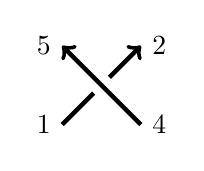
\begin{tikzpicture}
    \draw[->, ultra thick] (1,0) -- (0,1) node[pos=0, right] {4} node[pos=1, left] {5};
    \draw[ultra thick] (0,0) -- (0.4,0.4) node[pos=0, left] {1};
    \draw[->, ultra thick] (0.6,0.6) -- (1,1) node[pos=1, right] {2};
\end{tikzpicture}

\hspace{2mm}
\raisebox{6mm}{$\longrightarrow$}
\hspace{2mm}

\raisebox{5.5mm}{\Large$A$}
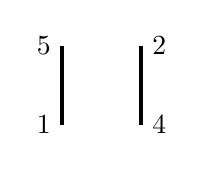
\begin{tikzpicture}
    \draw[ultra thick] (0,0) -- (0,1) node[pos=0, left] {1} node[pos=1, left] {5};
    \draw[ultra thick] (1,0) -- (1,1) node[pos=0, right] {4} node[pos=1, right] {2};
\end{tikzpicture}

\hspace{2mm}
\raisebox{6mm}{$+$}
\hspace{2mm}

\raisebox{5.5mm}{\Large$A^{-1}$}
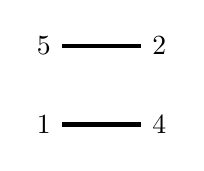
\begin{tikzpicture}
    \draw[ultra thick] (0,0) -- (1,0) node[pos=0, left] {1} node[pos=1, right] {4};
    \draw[ultra thick] (0,1) -- (1,1) node[pos=0, left] {5} node[pos=1, right] {2};
\end{tikzpicture}